% Digital Logic Lab 3 Report
% Created: 2020-02-01, Alexander Noll; Jonah Trahan

%==========================================================
%=========== Document Setup  ==============================

% Formatting defined by class file
\documentclass[11pt]{article}

% ---- Document formatting ----
\usepackage[margin=1in]{geometry}	% Narrower margins
\usepackage{booktabs}				% Nice formatting of tables
\usepackage{graphicx}				% Ability to include graphics

%\setlength\parindent{0pt}	% Do not indent first line of paragraphs 
\usepackage[parfill]{parskip}		% Line space b/w paragraphs
%	parfill option prevents last line of pgrph from being fully justified

% Parskip package adds too much space around titles, fix with this
\RequirePackage{titlesec}
\titlespacing\section{0pt}{8pt plus 4pt minus 2pt}{3pt plus 2pt minus 2pt}
\titlespacing\subsection{0pt}{4pt plus 4pt minus 2pt}{-2pt plus 2pt minus 2pt}
\titlespacing\subsubsection{0pt}{2pt plus 4pt minus 2pt}{-6pt plus 2pt minus 2pt}

% ---- Hyperlinks ----
\usepackage[colorlinks=true,urlcolor=blue]{hyperref}	% For URL's. Automatically links internal references.

% ---- Code listings ----
\usepackage{listings} 					% Nice code layout and inclusion
\usepackage[usenames,dvipsnames]{xcolor}	% Colors (needs to be defined before using colors)

% Define custom colors for listings
\definecolor{listinggray}{gray}{0.98}		% Listings background color
\definecolor{rulegray}{gray}{0.7}			% Listings rule/frame color

% Style for Verilog
\lstdefinestyle{Verilog}{
	language=Verilog,					% Verilog
	backgroundcolor=\color{listinggray},	% light gray background
	rulecolor=\color{blue}, 			% blue frame lines
	frame=tb,							% lines above & below
	linewidth=\columnwidth, 			% set line width
	basicstyle=\small\ttfamily,	% basic font style that is used for the code	
	breaklines=true, 					% allow breaking across columns/pages
	tabsize=3,							% set tab size
	commentstyle=\color{gray},	% comments in italic 
	stringstyle=\upshape,				% strings are printed in normal font
	showspaces=false,					% don't underscore spaces
}

% How to use: \Verilog[listing_options]{file}
\newcommand{\Verilog}[2][]{%
	\lstinputlisting[style=Verilog,#1]{#2}
}




%======================================================
%=========== Body  ====================================
\begin{document}

\title{ELC 2137 Lab 3: Adders}
\author{Alexander Noll, Jonah Trahan}

\maketitle


\section*{Summary}

The lab was designed to put into practice logic gate in order to perform basic mathematical functions. Using only AND and XOR gates a half, full, and 2-bit full adder were created and tested. The construction was planned using foreknowledge of Boolean arithmetic and truth tables.


\section*{Q\&A}

Which gates could be used for combining carry bits?

OR or XOR gates can used to add carry bits. We should use XOR gates as they minimize the number of different gates needed and work functionally the same as an OR gate. See Table 1 for exhaustive proof in truth table.

\clearpage
\section*{Results}


\begin{figure}[!hb]\centering
	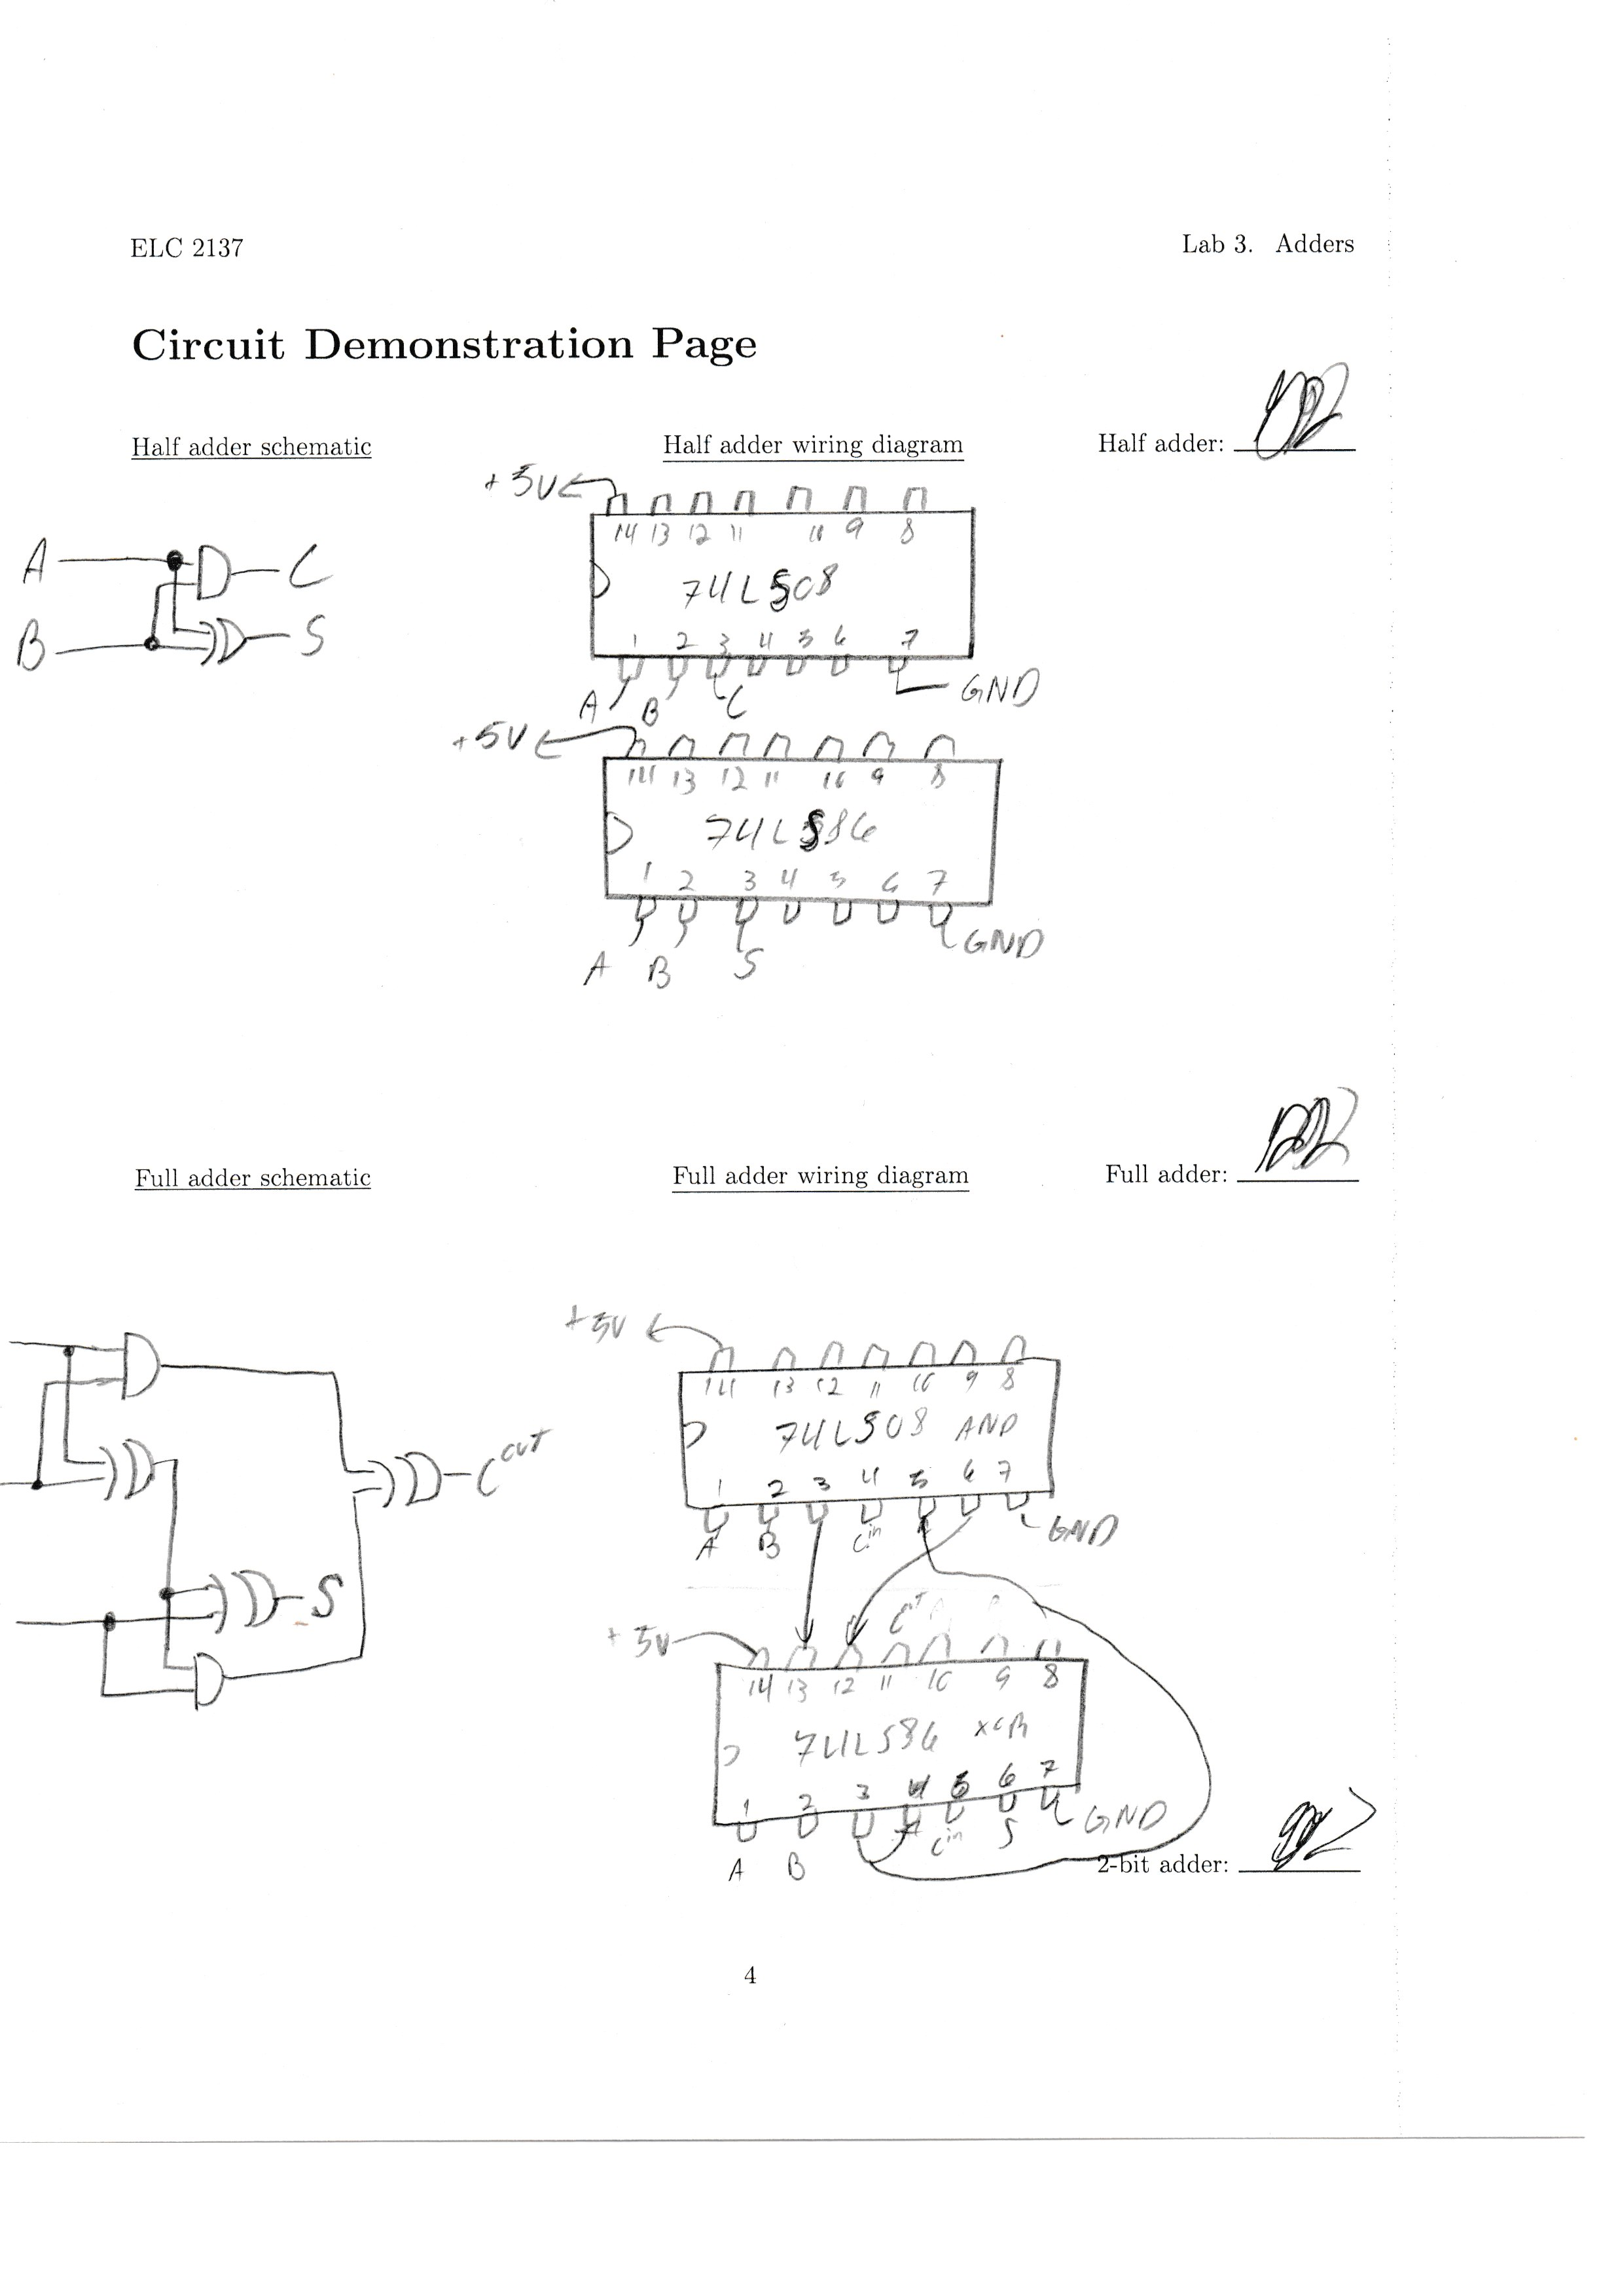
\includegraphics[width=.75\textwidth]{DiagramSheet} \caption{Circuit demonstration page with Half and full adder schematics and wiring diagrams. The document also includes instructor initials for the completion of each adder type}
\end{figure}

\begin{figure}[!htb]\centering
	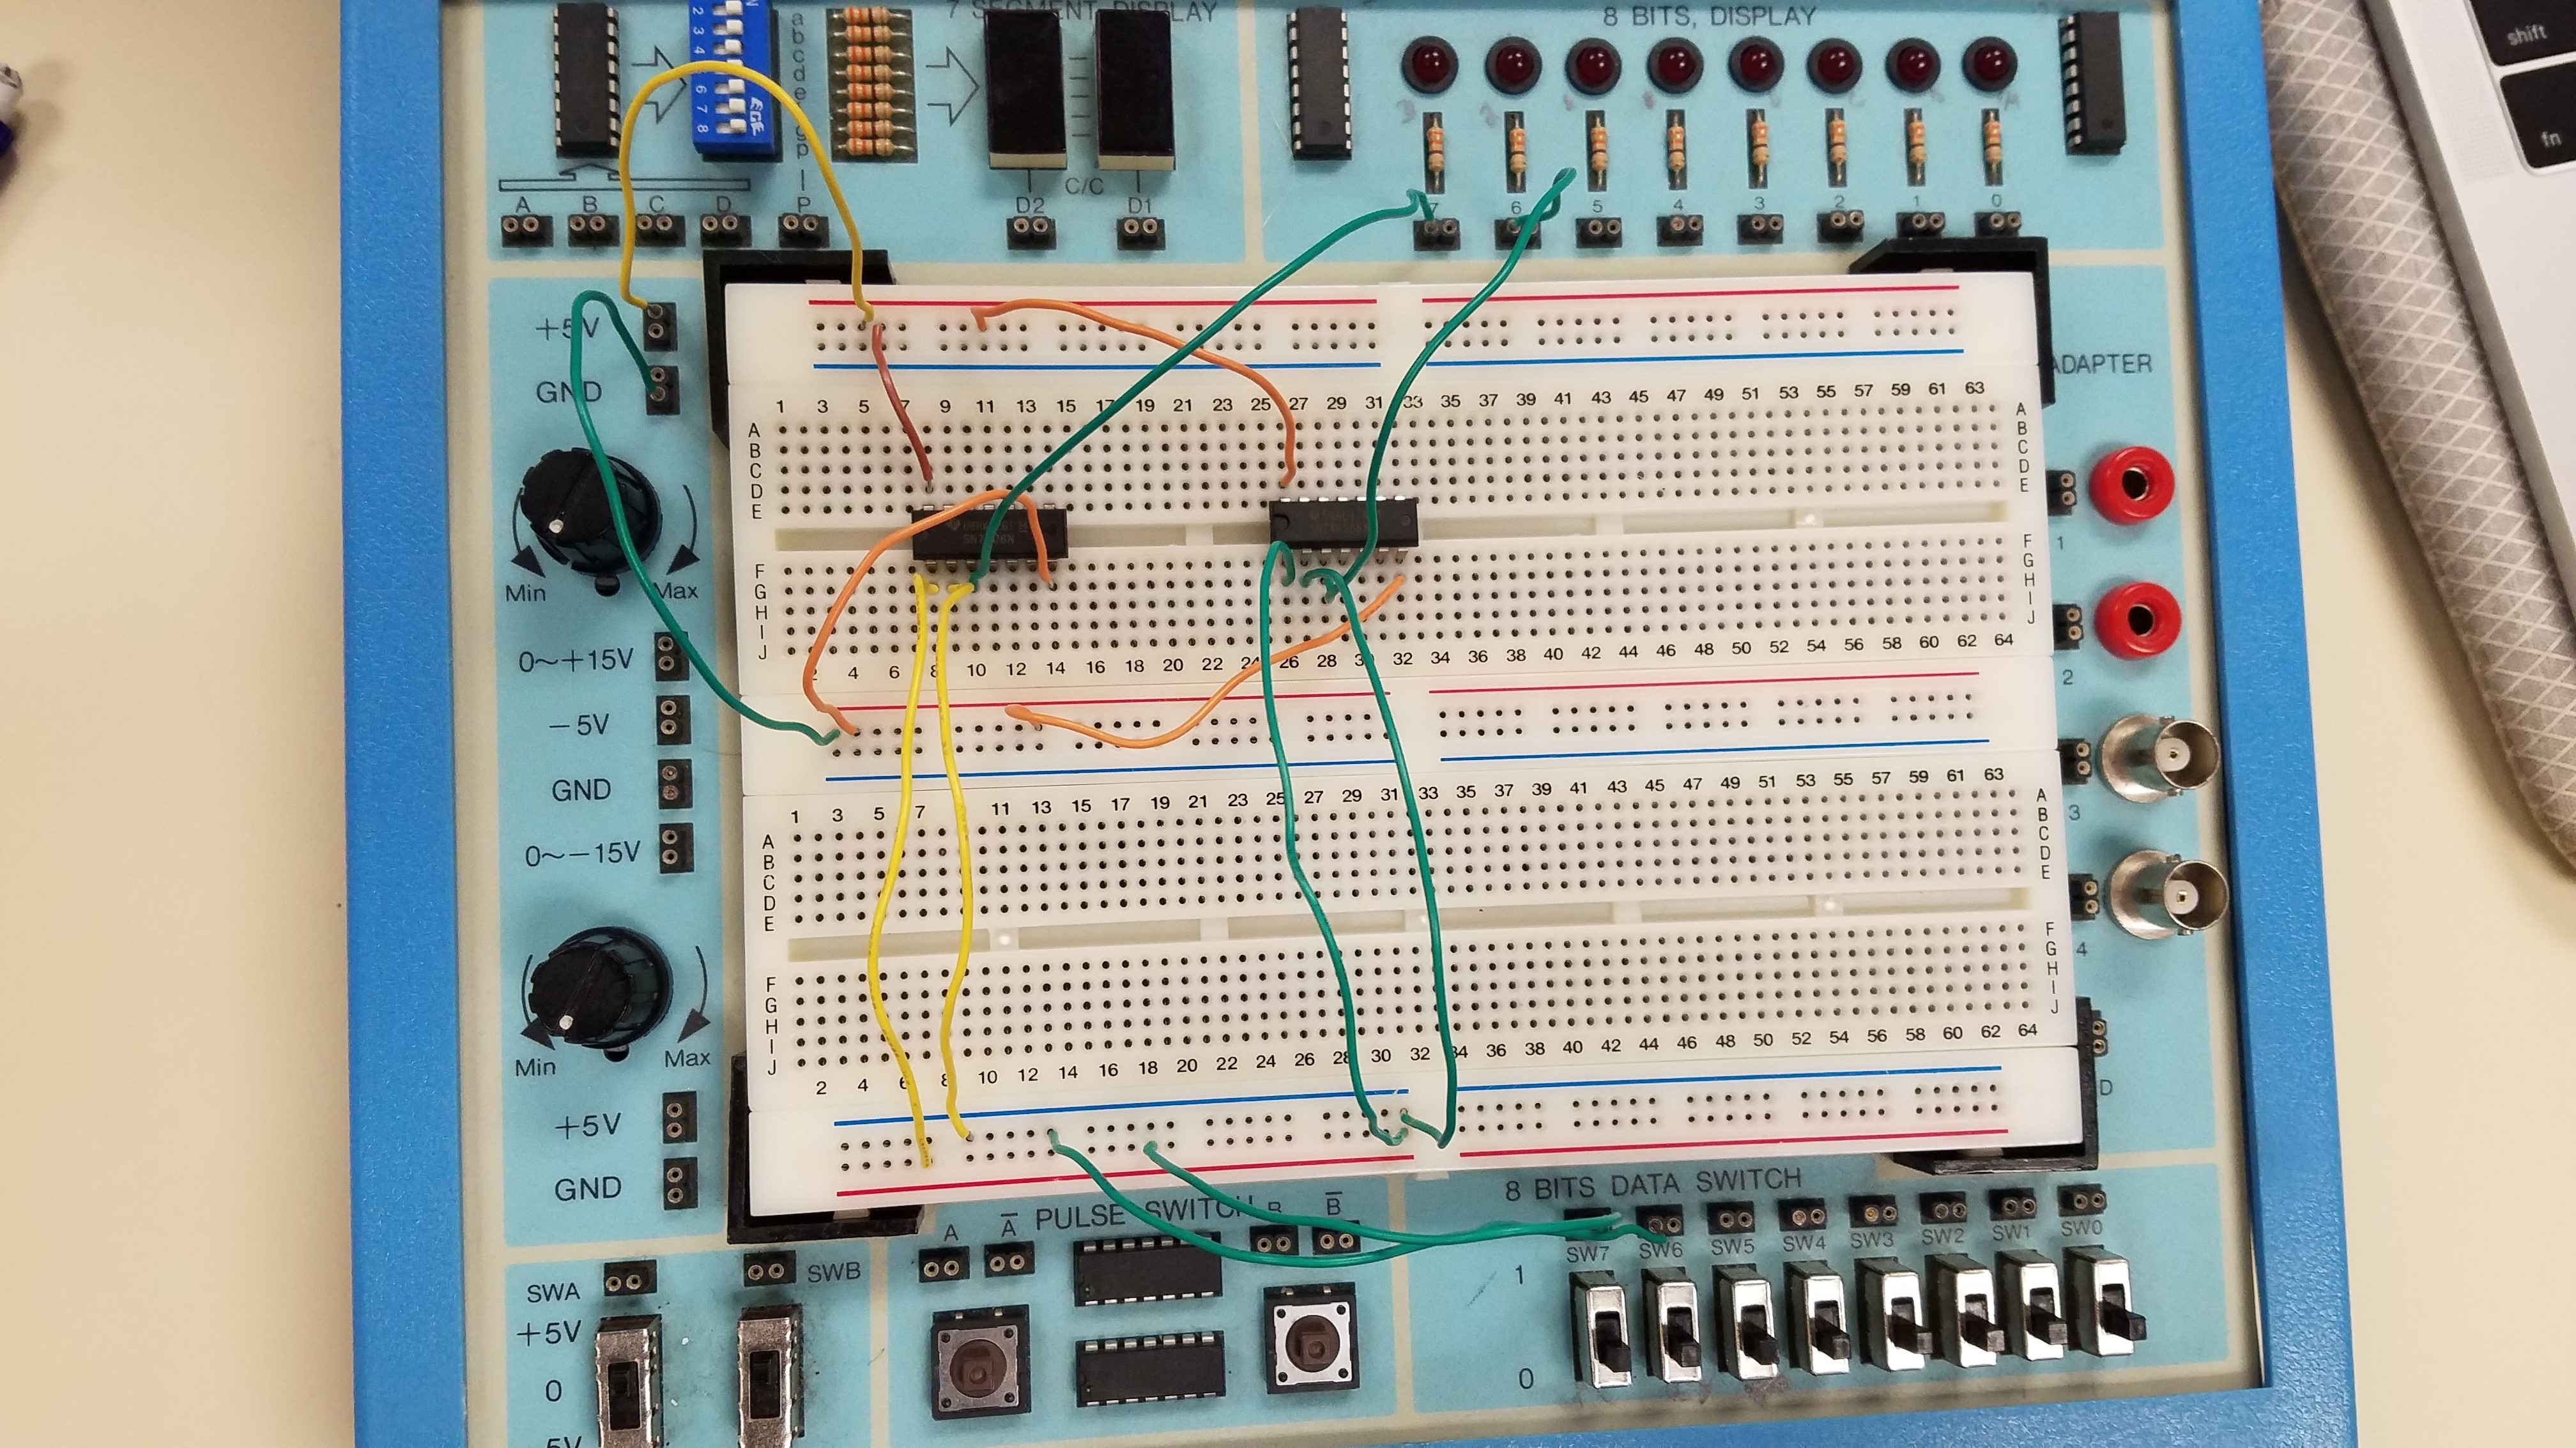
\includegraphics[width=.5\textwidth]{HalfAdder} \caption{Image of constructed Half Adder.}
\end{figure}

\begin{figure}[!htb]\centering
	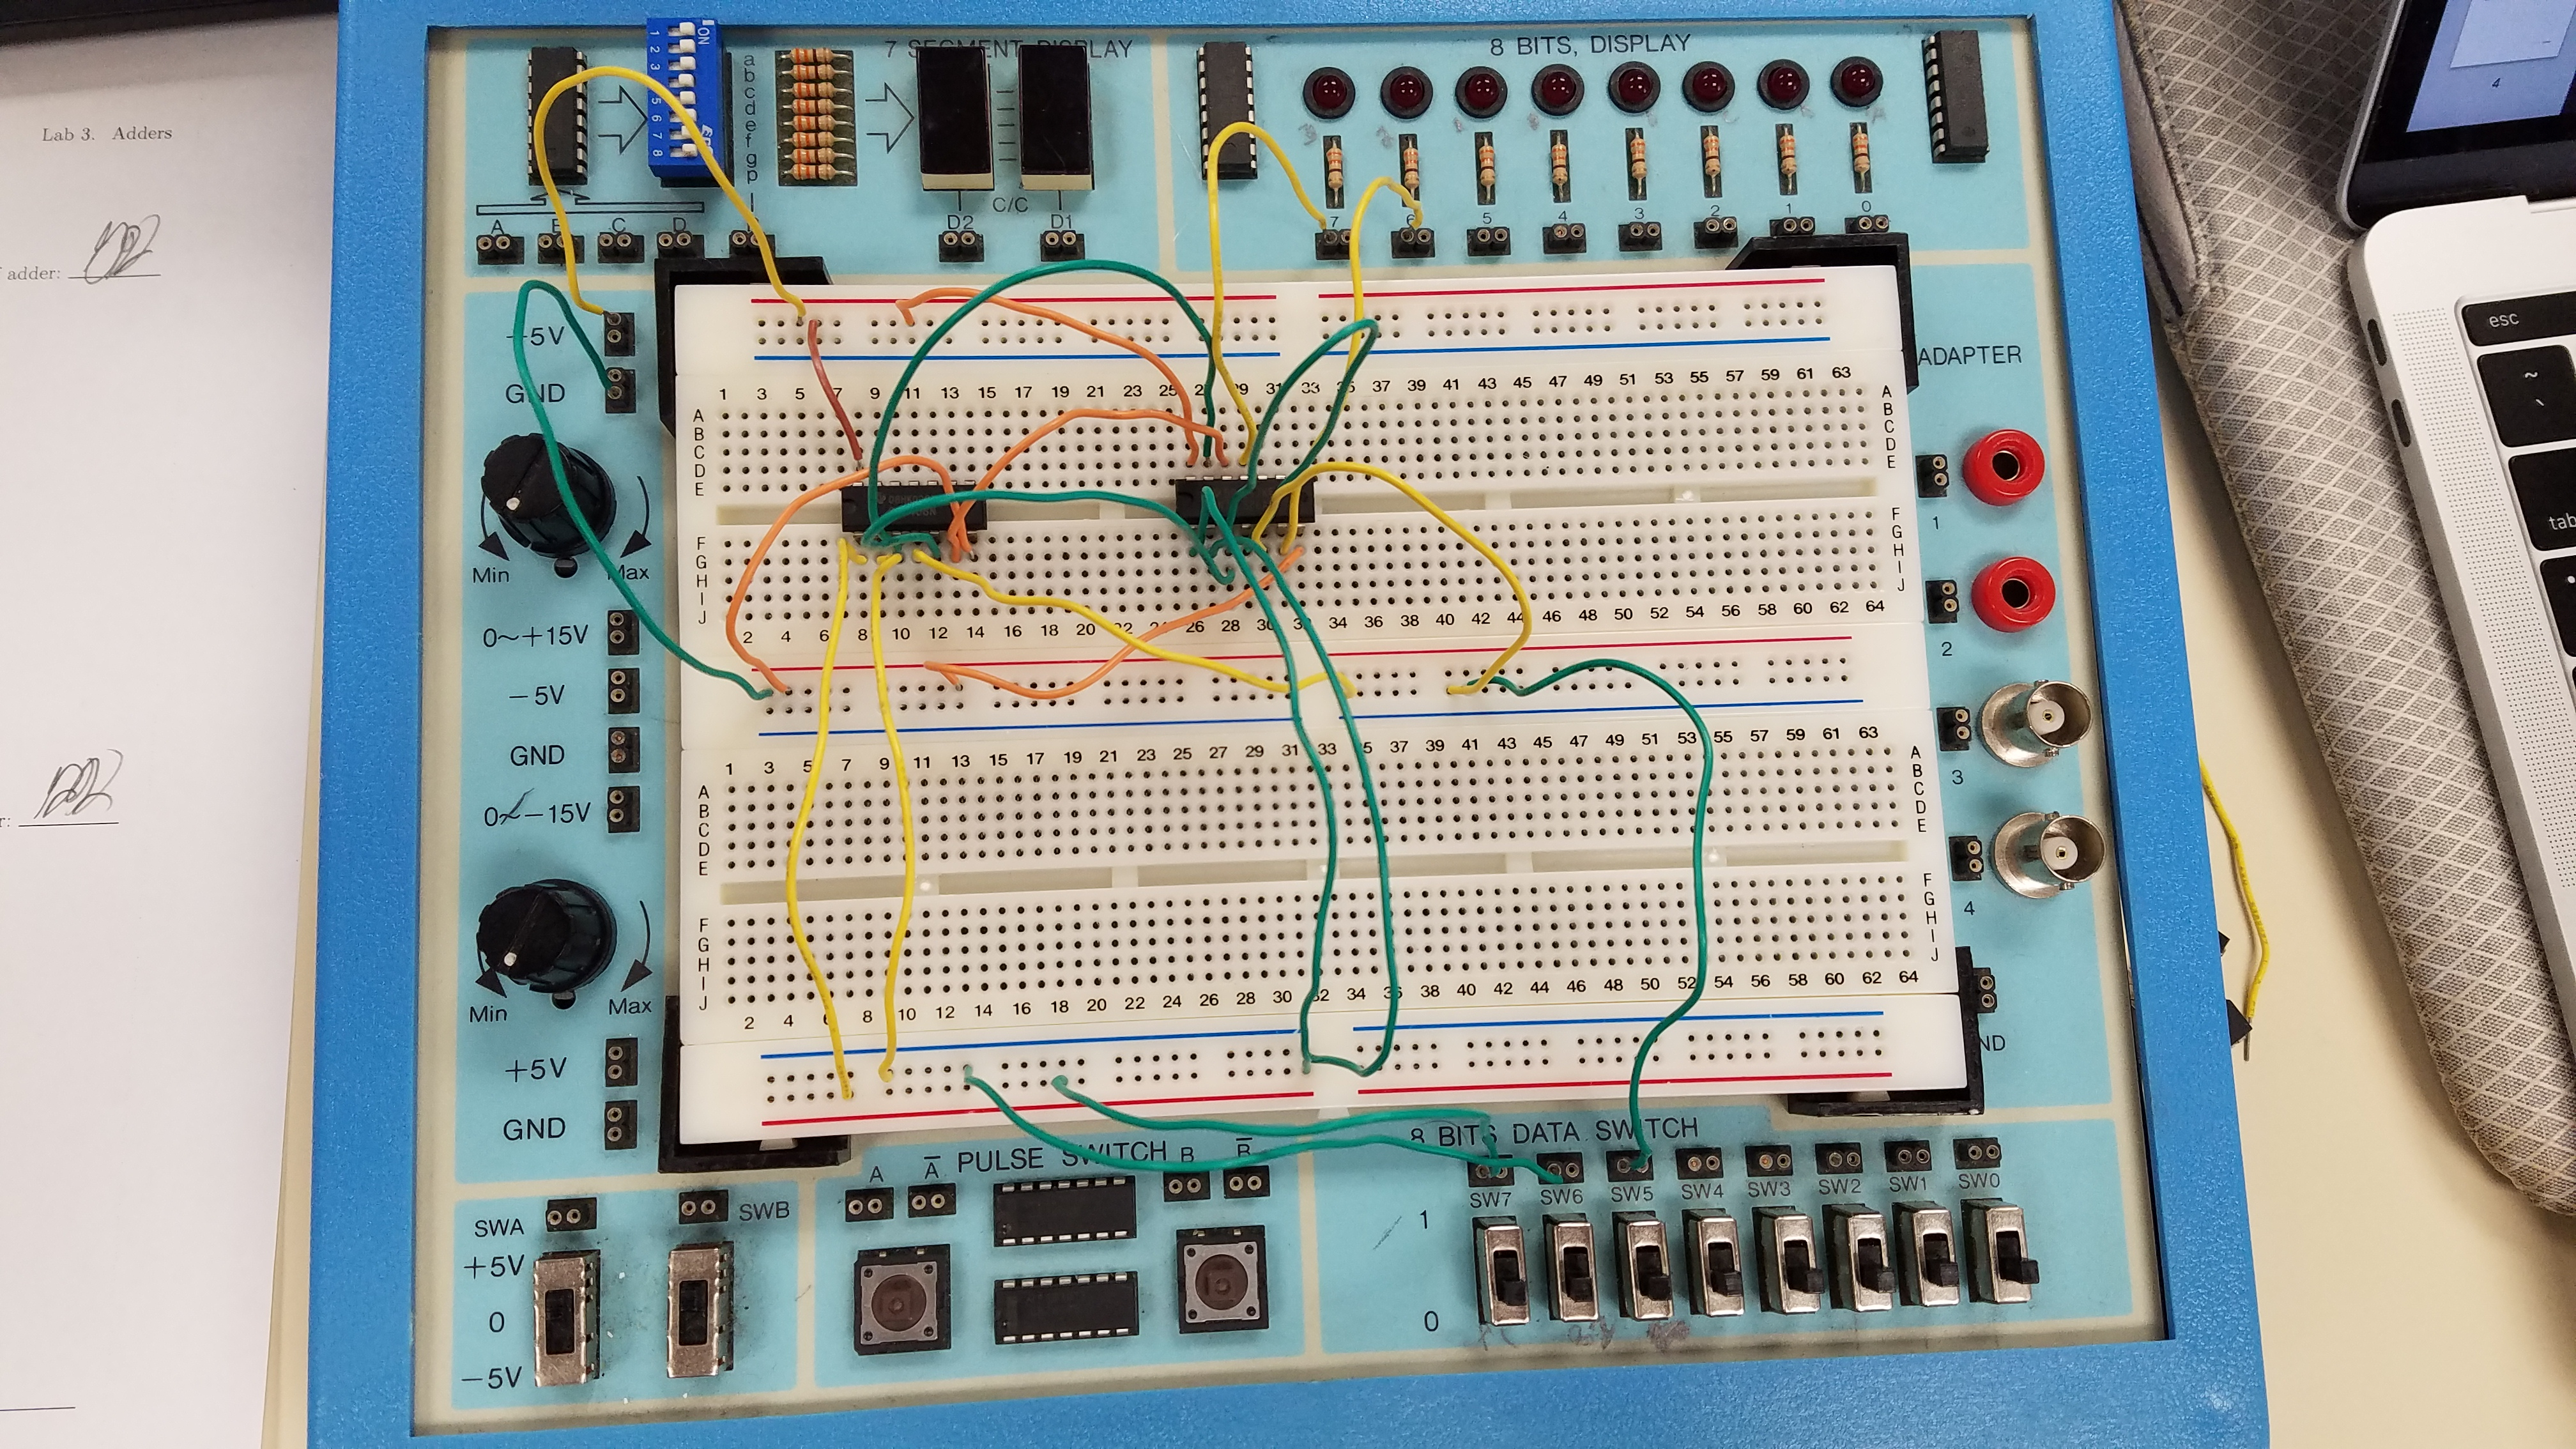
\includegraphics[width=.5\textwidth]{FullAdder} \caption{Image of constructed full adder.}
\end{figure}

\begin{figure}[!htb]\centering
	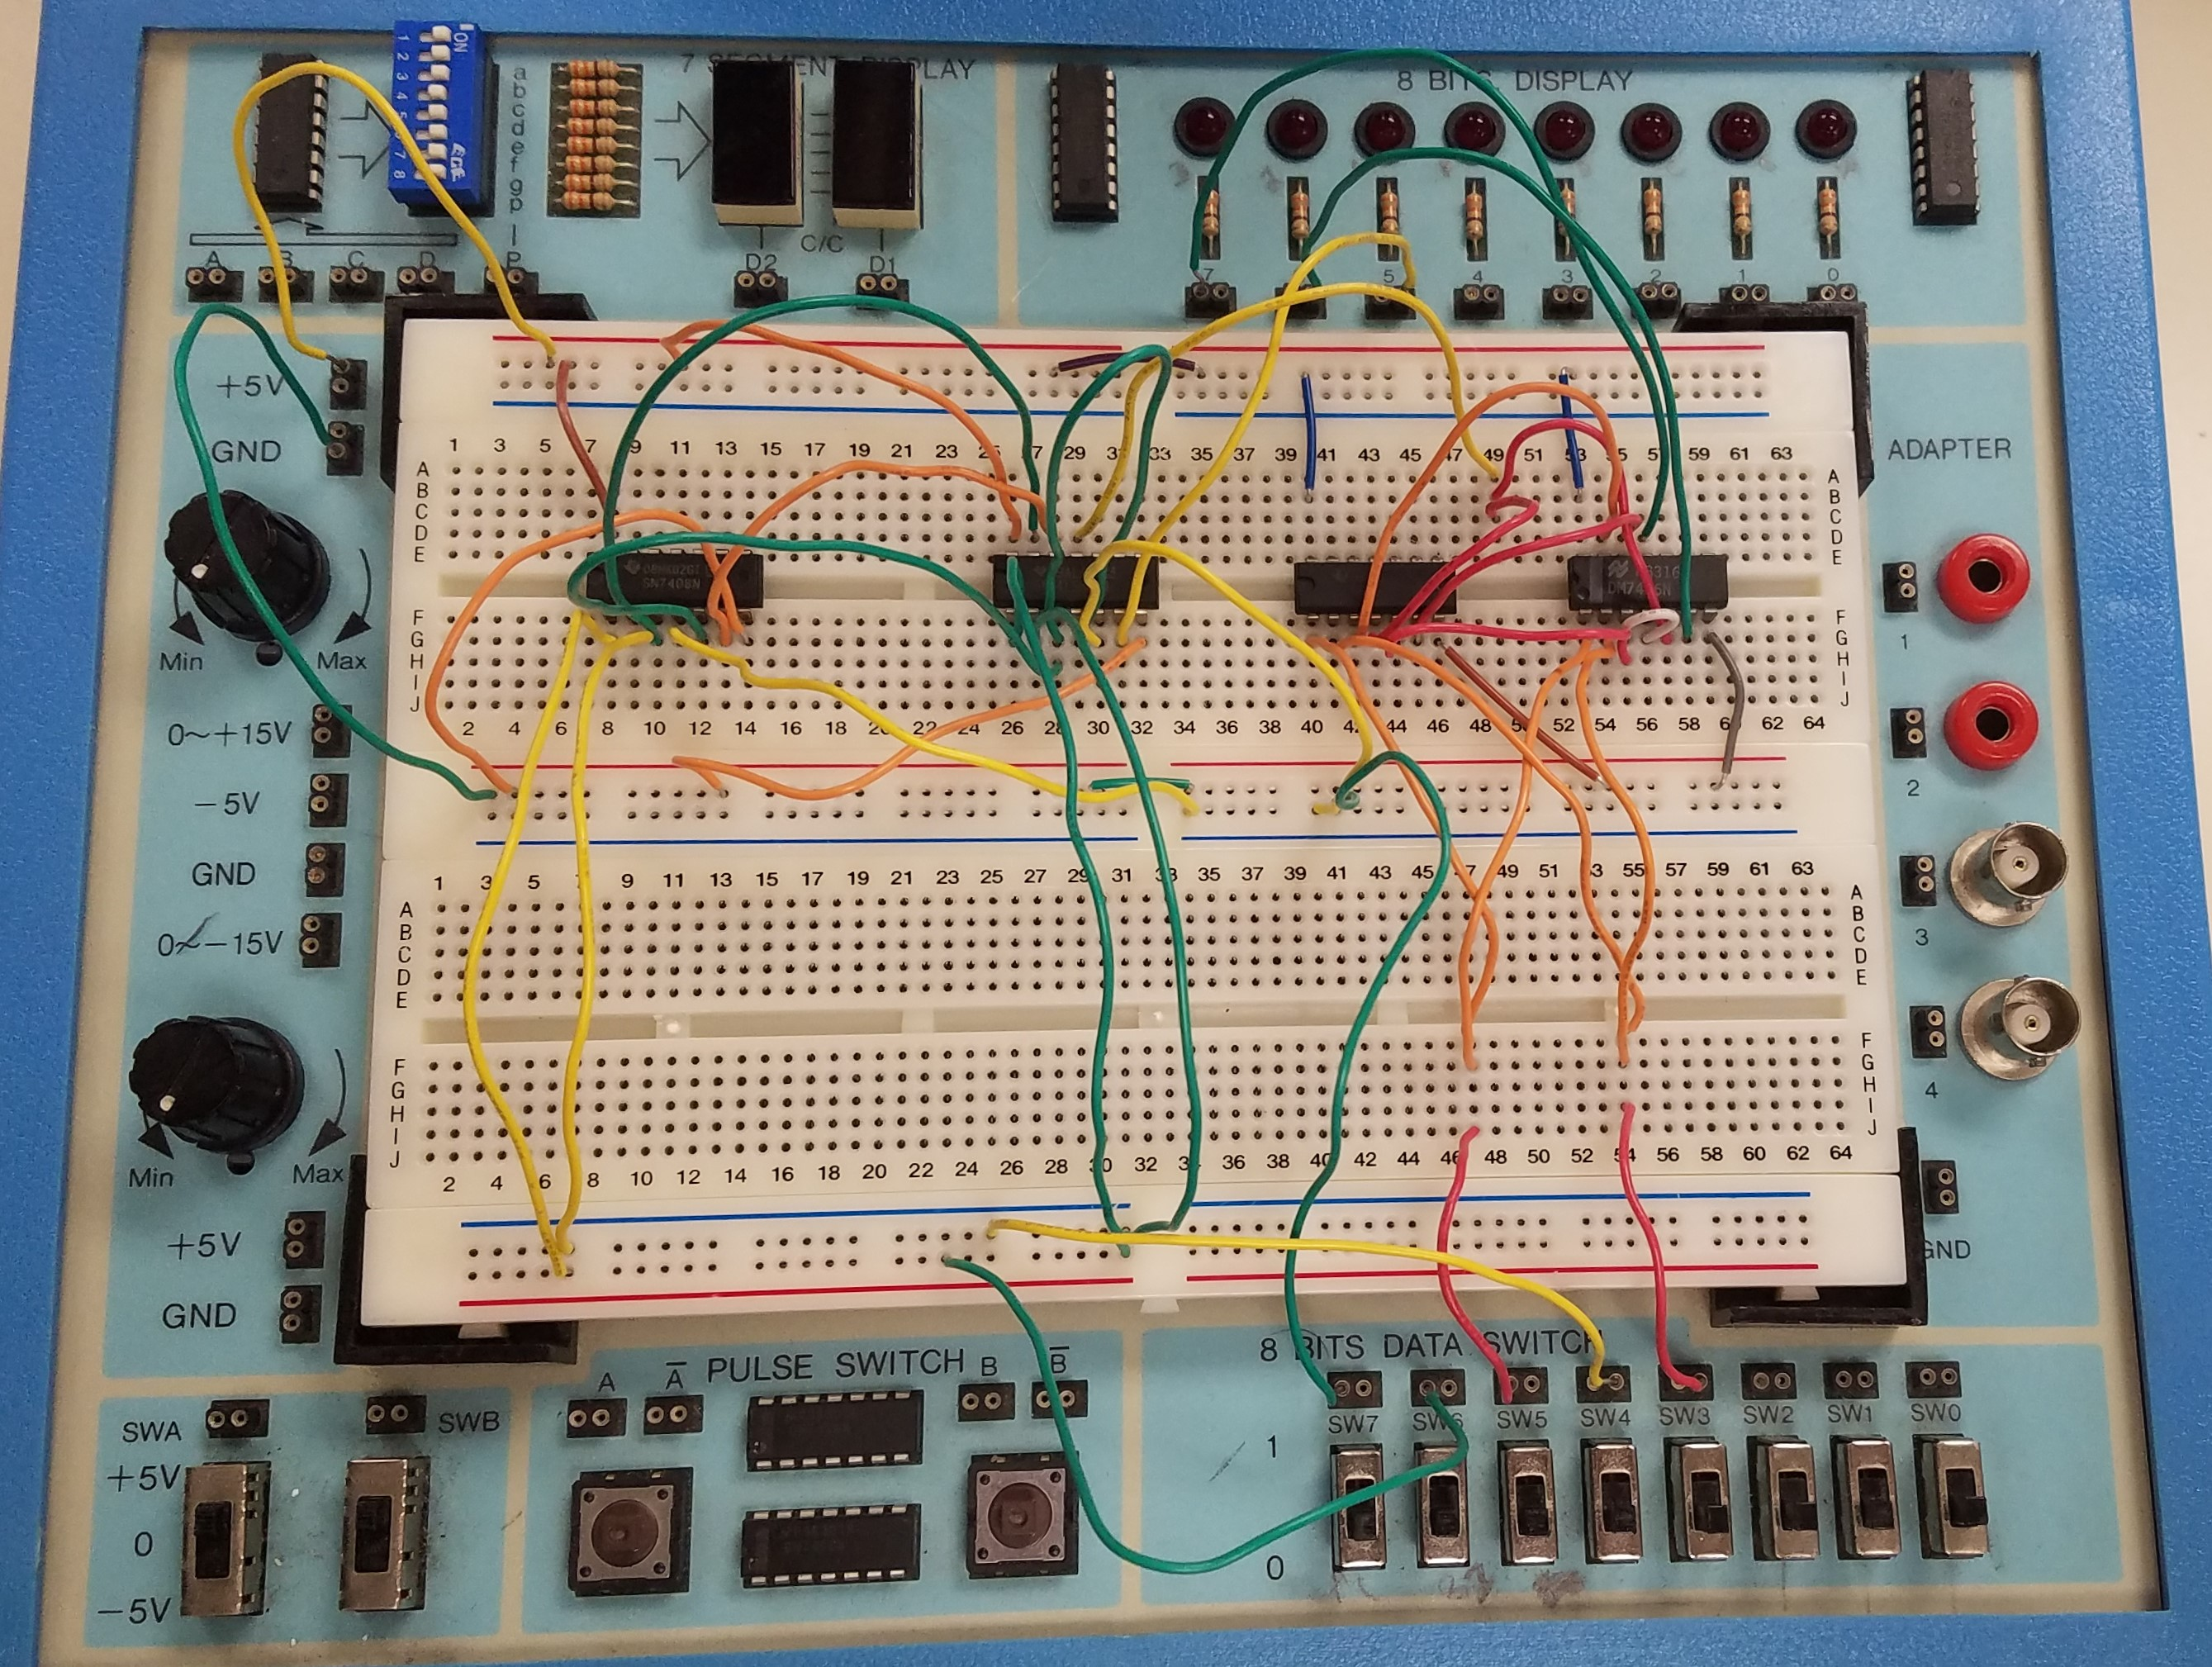
\includegraphics[width=.5\textwidth]{2BitAdder} \caption{Image of constructed 2 bit full adder}
\end{figure}

\begin{table}[!htb]\centering\caption{Carry Bit Addition Truth Table}\label{tbl:example_table}\begin{tabular}{c|c|c|c|c}\toprule Cin & Half Adder Sum (S) & S*Cin (X) & C & Cout(S XOR C) \\\midrule0 & 0 & 0 & 0 & 0  \\0 & 1 & 0 & 0 & 0 \\0 & 0 & 0 & 1 & 1 \\1 & 0 & 0 & 0 & 0 \\1 & 1 & 1 & 0 & 1 \\1 & 0 & 0 & 1 & 1 \\\bottomrule\end{tabular} \caption{The Truth Table demonstrates through exhaustive proof that no matter the inputs both carry digits X and C will never both be 1 and the XOR gate can always add them as an OR gate would.*}

* Two repeated lines in the truth table were omitted as they only exist as a consequence of the intermediate carry bit, C, being unable to be 1 when S=1 and visa versa. This is due to S being the result of an AND gate of only two one-bit inputs and thus the largest binary out is 10. The rightmost bit being the carry bit C, and the leftmost bit being S. 
\end{table}

\end{document}
